\documentclass[letterpaper]{article}
\usepackage[top=1.0in,bottom=1.0in,left=1.0in,right=1.0in]{geometry}
\usepackage{verbatim}
\usepackage{amssymb}
\usepackage{graphicx}
\usepackage{svg}
\usepackage{longtable}
\usepackage{amsfonts}
\usepackage{amsmath}
\usepackage{hyperref}
\usepackage{float}
\usepackage{caption}
\usepackage{xcolor}
\def\thesection       {\arabic{section}}
\def\thesubsection     {\thesection.\alph{subsection}}

\author{Zoe Richter
        \\ \href{mailto:zrichte2@illinois.edu}{\texttt{zrichte2@illinois.edu}}
}
\title{Learn Some Programming and Scream Less\thanks{probably}}
\begin{document}
\maketitle

\section{Keywords}

This is a list of terms you may see often.

\begin{itemize}
\item GUI: Graphical User Interface.  This is the term for the user-friendly interfaces that often use mouse clicks and images to get things done.  For example, the file explorer on your computer is a GUI for manipulating your files (the alternative being to directly mess with them in a terminal).
\item supress the output: if your code is supressing the output of a line of code, that means it won't print its results to the screen.
\item syntax: in programming, syntax refers to the punctuation and general "grammar" rules of the language.  For example, MatLab syntax requires a ; at the end of each line to supress the output, but Python defaults to supressing it.


\end{itemize}

\section{What is This?}

Computer programming is a skill that can be applied in some capacity to most any field.  For nuclear applications, computers often help by either automating a process, or by simulating systems that are too costly or hazardous to be able to easily build in a lab (think of trying to test things pertaining to reactors - they're big, really hot, highly pressurized, radioactive, and very expensive to make).\\

In the hands-on lesson, you worked with MatLab specifically.  Matlab is great for a lot of engineering applications, but you might not see it used outside of those applications (and it costs money, which makes me cry).\\

Below, I've collected some resources for teaching yourself programming, and some general tips that I've found helpful.

\section{What is a Linux?}

Chances are, your operating system is either Windows or Mac.  In my experience, either of these are great for general use.  They're user friendly, and most any software will be compatible with them.  However, when it comes to any sort of programming work, I prefer to use Linux.  For example, my personal laptop is running Windows, while my work computer is currently running Ubuntu 16.04.  The reason for this is that Linux (and Mac, but I still prefer Linux for work) actually intends for you to use the terminal.  You should also consider what version of your OS you need.  For most projects, the most recent "stable" build is perfect.  It's as up-to-date as possible without having a bunch of bugs.  For some things, though, such as software creation, you might find that you want the "bleeding-edge" of your OS of choice.  This is the most recent version, but also comes with more issues, as the "bleeding-edge" is still being tested and patched.\\

If you're stuck with Windows, don't despair.  You can use an emulator, such as GitBash, to get these features on your system.  In the next section, the lesson I refer to gives other options for Windows users in the "getting started" section.

\section{Hello, I am Scared of the Terminal}

This is a real-life terminal with real-life files where my real-life fingers input real-life commands.
\begin{figure}[H]
  \centering
  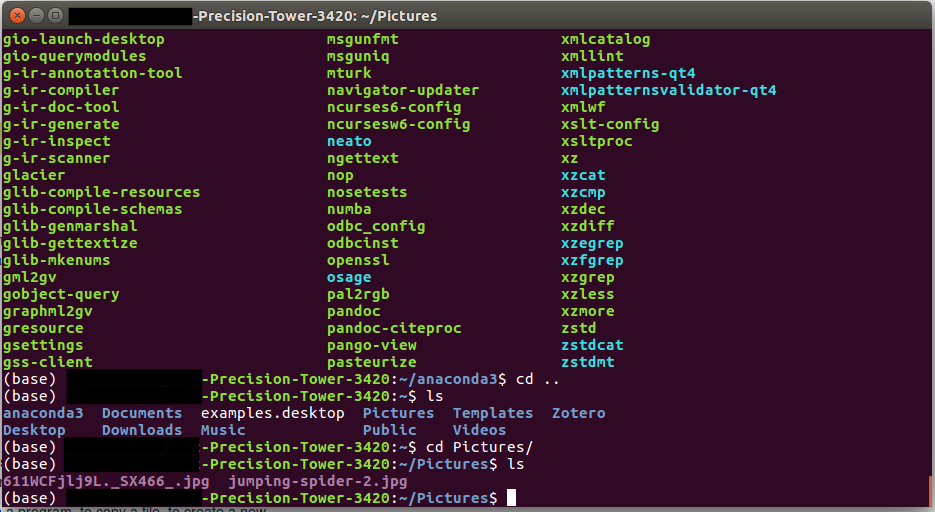
\includegraphics[width=1.0\linewidth]{wowterminal.png}
  \captionof{figure}{A Picture of a Terminal}
  \label{fig:fig1}
\end{figure}

I can already hear some of you crying.  Dry your eyes.  Movies make hacking look cool and difficult because real programming is often a very unhappy person yelling at their poor computer.\\

Coding is a skill I definitely think anyone can teach themselves, with what I would call an average amount of technological literacy.  I, personally, started off with lessons from \href{https://software-carpentry.org/lessons/}{software-carpentry}.  For Unix, you can look at \href{http://swcarpentry.github.io/shell-novice/}{this one}.  Throughout the rest of this document, I'll leave links to relevant lessons on their website.\\

In general, I've found that a lot of people (myself included) struggle at first because they view the terminal as some sort of eldritch entity that will eat their computer if they use the wrong words.  And while you certainly \emph{could} bork your computer, many commands you'll be using won't do anything at all if you enter it wrong.  You need to start being more sure of what you're doing when you start doing things to rename or delete files, especially in bulk.

\section{Git: Please Use This One Day It Will Save Your Life}

Consider the following.  Twenty page term paper.  You finished it with an hour to spare.  You trip on your way to class, and your laptop tumbles into the path of an oncoming bus, crushing it and your dreams of passing to dust.\\

But never fear, Git is here!  Git is a repository system that will save "versions" of your files as you commit their changes to git's logs.  Instead of saving multiple versions of a file as different files, you can have one current version of it, and, if you decide that a previous version is better than what you currently have, you can revert to any previously saved file state.\\

Think of it like having multiple saves of a video game.  You might save your game just before choosing whether or not to jump off a cliff to see if there's fall damage.  Once you jump off and hit the ground, you save to a different file, realizing that there isn't fall damage, and your dragon-slayer isn't a pancake.  But after running around at the bottom of the cliff for a bit, you realize that you can't jump your way back out, and there isn't anything down here but low-poly bushes.  This isn't ideal, so you load up the save from before you jumped off the cliff, and do something else instead, like pick flowers.  In the same way, you might tell git to save the state of a report before you start making a bunch of changes.  If you later decide you don't like these changes, you can revert to the file state before you started messing with things.\\

But, while this saves you if a less-than-stelar team member goes through your 50 page report and changes all the "cannot"s to "can not", it doesn't save you from the bus-scenario mentioned earlier.  That is because git is a local repository - it only exists on your personal machine.  To save your project elsewhere, you want to use a remote repository such as GitHub.  GitHub is a service for saving and maintaining a git repository on a remote server.  It saves all of your files, tracks changes, and provides various tools for collaborating with other people.  So, when your laptop gets run over by a bus, you can simply login to your GitHub on another computer, and access the files there, like nothing happened.\\

This has been a fairly simplified explanation of how git works.  To learn how to use it, and how it works in more detail, I would once again refer you to software-carpentry's lesson on \href{http://swcarpentry.github.io/git-novice/}{git}.

\section{Latex: Make Pretty Reports}

Latex is a language used to create pdfs.  It's actually what was used to make this report.  It uses a filetype exclusive to Latex, a .tex file.  Latex requires the use of a program such as Texmaker to run these .tex files, and compile them into a pdf.\\
\\
Latex is pretty useful for a few reasons.  For one, I think it's probably considered more "professional" than something like Microsoft Word.  It also makes citations, especially in-text citations, much easier.  Also, for the purpose of writing a technical report, Latex allows you to enter and edit mathematical equations much quicker than the GUI equation editor in Word.  You can also generate a file for your bibliography (a .bib) and put it into your .tex file.  When it compiles, it will automatically format the bibliography for you.
\\
\\
There isn't a Latex tutorial on software-carpentry, but once you get the basics down, you can figure out how to do most things by googling it.  To give an example, the repository that holds all of this includes the.tex file I used to make this paper.  To get the needed software and packages, I, personally, used \href{https://miktex.org/about}{MikTex}.\\

\emph{This} \textcolor{teal}{sentence} \colorbox{green}{is to} \underline{\textbf{show}} {\LARGE{some}} {\tiny{cool}} \LaTeX \texttt{ formatting}.  You can also put math in the middle of a sentence, like this: $ \Delta + 5 = 10 ; \Delta = 5$.  Or, if you can do this:
\begin{align}
\Delta = \sqrt{x^{2} + \sum_{i = 0}^{5}y*i} \label{eq:eq1} \\
Given: x = 2, y = 3 \nonumber \\
\Delta = \sqrt{2^{2} + \sum_{i = 0}^{5}3*i} \label{eq:eq1.1} \\
\Delta = 7 \notag
\end{align}

\section{Python: I Don't Have a Snappy One-Liner}

Python is a very popular language.  It's free, open-source, and continually being updated and improved.  I would recommend that anyone interested in a STEM major take the time to learn the basics.  You can find some lessons on software-carpentry, such as \href{http://swcarpentry.github.io/python-novice-inflammation/}{this one} or \href{http://swcarpentry.github.io/python-novice-gapminder/}{this one}.  Since you'll likely be reading this after first being exposed to MatLab, I'll point out a few differences.\\

Python begins counting at 0.  MatLab starts at 1.  What does this mean?  Let's suppose you have a set of numbers, say $[2, 5, 8, 4, 7, 3]$.  Now, imagine that you need to ask your computer nicely to please give you the third number in the list - 8.  In python, this is:
\begin{verbatim}
a = [2, 5, 8, 4, 7, 3]

print(a[2])
\end{verbatim}
In MatLab, however, you'll be using this:
\begin{verbatim}
a = [2, 5, 8, 4, 7, 3];

disp(a(3))
\end{verbatim}
You might also notice that Python used [], but MatLab uses ().  There are many differences between these two languages in terms of their syntax.  However, the general idea of what something like a while or for loop is, and what it should do, won't change between languages.  So, while you may have to learn the specific way to write something in a new programming language, once you've learned your basics in one language, it becomes much easier to pick up the next one.

\section{Some Final Advice (From People Who are not Me)}

When I started making this, I asked other people in the field for advice they thought would help a fledgling programmer.  Here are the answers:

\begin{itemize}

\item \href{https://www.python.org/dev/peps/pep-0020/}{The Zen of Python}
\item Here is a link to a presentation by NPRE @ UIUC's Dr. Huff on \href{https://katyhuff.github.io/2018-12-22-mumbai/#/}{best practices}.  She also helps out with software carpentry lessons.
\item Speaking of software carpentry, there are resources on that website far beyond what I linked.  There are more lessons on the lessons page, and additional resources to be found elsewhere on the site.
\item "One thing I had to learn was to assume the user is intelligent. Some of the things that I have written in my free time have done excessive error catching which wasted a lot of time." -Nathan Bartholomew
\item "python -m pdb" - Teddy Bae.  ((This is in reference to the Python debugger interface.  Google python pdb and you'll find more on it.))
\item "Don't worry about having "necessary" skills, a lot of the fun is figuring things out. Everything you need to know can be found on the internet." - Sam Dotson
\end{itemize}

Some extra bits of advice I'd give:

\begin{itemize}

\item When programing, if you have a long and complicated formula to put in, break it up into smaller terms
\item When making functions, having more functions that are smaller is better than one big function that does everything
\item Looking at someone else's code usually sucks.  This will apply to looking at your own code after about two weeks.  Be kind to your friends, and to future you.  Give variables clear names.
\item There is a format guideline for Python, \href{https://www.python.org/dev/peps/pep-0008/}{pep8}, that gives specific directions for things like whether or not you should put a space after a comma.   Most of these things can be fixed automatically when you're done with your program with an auto pep8 tool.  However, pep8 also limits your lines to being less than 80 characters.  Auto-pep8-ifiers can't intelligently split up lines of code for you in my experience, so I would recommend keeping the lines under 80 characters when you're first writing it.
\item Consider making a playlist of music to zone out to while you work.  It makes things more enjoyable, and can help you tune out the rest of the world.
\item For MatLab help, I've found that the MathWorks documentation is a great help.  For Python help, I would start by looking at the documentation for the function you're having trouble with.  If, instead, you're just trying to figure out how to do some specific, kinda weird thing with Python, my best advice is to google what you want to do, and read all the StackExchange topics that sound sorta like what you want to do.  It's helped me every time.  While we're at it:
\item Make a StackExchange account.  It's super helpful.
\item If you have a bug and you can't figure it out, try rubber duckie coding.  Sometimes, when a bit of code has a stubborn error you just can't solve, the best thing to do is to talk out your code, and it can be especially helpful to explain what your code is doing, line-by-line, to someone else.  But, if you're a nerd like me, you might also be a recluse, and not have a person on hand to explain 300 lines of python to.  That's where the rubber duckie comes in.  It's a friendly inanimate object you can explain your code to, and, if you get mad at it, you can squish it and the rubber duckie will be just fine.  The author of this paper is not responsible for damages caused by thrown rubber duckies.
\end{itemize}

\section{Credit Where Credit is Due}

I've collected advice and tips from much of my personal experience learning to code here, but some of my friends and colleagues were kind enough to give some of their own advice, in the section above.  In addition, everything I learned starting out was with software carpentry, and while I've already linked to them a few times, I'd like to give another thanks to the folks that make all those free lessons.  You guys are the bee's knees.
\end{document}